%%
%% This is file `sample-authordraft.tex',
%% generated with the docstrip utility.
%%
%% The original source files were:
%%
%% samples.dtx  (with options: `authordraft')
%% 
%% IMPORTANT NOTICE:
%% 
%% For the copyright see the source file.
%% 
%% Any modified versions of this file must be renamed
%% with new filenames distinct from sample-authordraft.tex.
%% 
%% For distribution of the original source see the terms
%% for copying and modification in the file samples.dtx.
%% 
%% This generated file may be distributed as long as the
%% original source files, as listed above, are part of the
%% same distribution. (The sources need not necessarily be
%% in the same archive or directory.)
%%
%% The first command in your LaTeX source must be the \documentclass command.
\documentclass[sigconf,authordraft]{acmart}

%%
%% \BibTeX command to typeset BibTeX logo in the docs
\AtBeginDocument{%
  \providecommand\BibTeX{{%
    \normalfont B\kern-0.5em{\scshape i\kern-0.25em b}\kern-0.8em\TeX}}}

%% Rights management information.  This information is sent to you
%% when you complete the rights form.  These commands have SAMPLE
%% values in them; it is your responsibility as an author to replace
%% the commands and values with those provided to you when you
%% complete the rights form.
\setcopyright{acmcopyright}
\copyrightyear{2020}
\acmYear{2020}
\acmDOI{10.1145/1122445.1122456}

%% These commands are for a PROCEEDINGS abstract or paper.
\acmConference[Woodstock '18]{Woodstock '18: ACM Symposium on Neural
  Gaze Detection}{June 03--05, 2018}{Woodstock, NY}
\acmBooktitle{Woodstock '18: ACM Symposium on Neural Gaze Detection,
  June 03--05, 2018, Woodstock, NY}
\acmPrice{15.00}
\acmISBN{978-1-4503-XXXX-X/18/06}

\usepackage{graphicx}
\usepackage{subfig}
\graphicspath{ {./media/} }

%%
%% Submission ID.
%% Use this when submitting an article to a sponsored event. You'll
%% receive a unique submission ID from the organizers
%% of the event, and this ID should be used as the parameter to this command.
%%\acmSubmissionID{123-A56-BU3}

%%
%% The majority of ACM publications use numbered citations and
%% references.  The command \citestyle{authoryear} switches to the
%% "author year" style.

%%
%% end of the preamble, start of the body of the document source.
\begin{document}

%%
%% The "title" command has an optional parameter,
%% allowing the author to define a "short title" to be used in page headers.
\title{Point to Point Communication and Collective MPI Performance Test}

%%
%% The "author" command and its associated commands are used to define
%% the authors and their affiliations.
%% Of note is the shared affiliation of the first two authors, and the
%% "authornote" and "authornotemark" commands
%% used to denote shared contribution to the research.
\author{Yitao Shen}
\affiliation{%
  \institution{Rensselaer Polytechnic Institute}
  \streetaddress{110 8th Street}
  \city{Troy}
  \state{NY, 12180}
}
\email{larst@affiliation.org}

\author{Jinqiang Jiang}
\affiliation{%
  \institution{Rensselaer Polytechnic Institute}
  \streetaddress{110 8th Street}
  \city{Troy}
  \state{NY, 12180}
}
\email{larst@affiliation.org}

\author{Chau-Lin Huang}
\affiliation{%
  \institution{Rensselaer Polytechnic Institute}
  \streetaddress{110 8th Street}
  \city{Troy}
  \state{NY, 12180}
}
\email{huangc11@rpi.edu}

\author{Lorson Blair}
\affiliation{%
  \institution{Rensselaer Polytechnic Institute}
  \streetaddress{110 8th Street}
  \city{Troy}
  \state{NY, 12180}
}
\email{larst@affiliation.org}



\author{Christopher D. Carothers}
\affiliation{%
  \institution{Rensselaer Polytechnic Institute}
  \streetaddress{110 8th Street}
  \city{Troy}
  \state{NY, 12180}
}
\email{chrisc@cs.rpi.edu}



%%
%% By default, the full list of authors will be used in the page
%% headers. Often, this list is too long, and will overlap
%% other information printed in the page headers. This command allows
%% the author to define a more concise list
%% of authors' names for this purpose.
\renewcommand{\shortauthors}{Yitao Shen, et al.}

%%
%% The abstract is a short summary of the work to be presented in the
%% article.
\begin{abstract}
  % This is the abstract

Communication among multiple nodes plays a critical role in the performance of High Performance Computing. MPI \cite{clarke1994mpi} offers a great number of libraries to maximize and test the communication performance in the parallel computing networks. The message passing has been observed to spend additional time in transfering information from one node to another, and several parallel models have been devised to properly describe the phenomenon, which in terms serve as criteria for future benchmarking. In this work, we build a collective MPI performance test to evaluate the performance among different models. To accomplish this, we have a parallel version of Game of Life program optimized with MPI communication scheme and CUDA for GPU parallelization. As far as the authors are concerned, this work could be the first intend to verify the networking perforamnce of a GPU-aided program in terms of different paralllel models. In terms of hardware, the benchmarking takes place on AiMOS \cite{aimos}, an eight petaflop supercomputer using a heterogenous system architecture built with IBM POWER9 CPUs and NVIDIA GPUs. On the software side, the program relies on IBM Spectrum MPI and NVidia CUDA math library \cite{aimosibm}.
\end{abstract}

%%
%% Keywords. The author(s) should pick words that accurately describe
%% the work being presented. Separate the keywords with commas.
\keywords{Parallel Computing, High Perforamnce Computing, CUDA, MPI}


%%
%% This command processes the author and affiliation and title
%% information and builds the first part of the formatted document.
\maketitle

\section{Introduction} \label{introduction}
% Performance Metrics







\section{Related Works} \label{relatedWorks}
% Related works

There are several works discussing the benchmarking of MPI performance on parallel systems using different libraries. Pje{\v{s}}ivac-Grbovi{\'c et al. \cite{pjevsivac2007performance} give a thorough overview of the parallel models, and compare the performances on inter-cluster MPI collective operations on two systems. The authors in the mentioned article also demontrate that the gap between the message sendings depends on the number of unique destination nodes.  

There are also works whose authors discuss the communication performance on the parallel version of Conway's Game of Life. L. Ma et al. \cite{ma2012performance} demonstrate the performance boosting by implementing the algorithm into its parallel counterpart. The article\'s author implemented the parallel program with OpenMP library, which takes advantage of the multithreading in the CPU rather than seeking time efficiency improvement from multi-node perspective.

In our work we referenced an open-source framework for implementing network benchmarks presented by T. Hoefler et al. \cite{hoefler2007netgauge} This framework seperate communication patterns from communication moddules which allows independently added benchmark types and network protocols. The authors also presented a LogGPS pattern \cite{hoefler2007low} which supports measurement of LogP and LogGP models parameters such as latency, overhead and gap per bytes over MPI.


\section{Game of Life as an Algorithm} \label{gol}
% Game of Life

The Game of Life as invented by the British mathematician John Horton Conway in 1970 \cite{gardener1970mathematical} is a cellular automaton. The algorithm is a zero-player game and as the game evolves throughout undetermined number of iterations, the outcome is determined by the given initial configuration. The game is taken place on a two-dimensional orthogonal grid of square cells. The cell status is atomic, that is it can only be found as alive or dead. Each cell's status is determined by eight adjacent neighboring cells. At each step in time, any cell with fewer than two live neighbors dies due to under-population. On the contrary, if the cell lives with two or three live neighbors survives to the next step. If there are more than three immediately adjacent cells, the cell perishes due to over-population. Lastly, the cell resucitates with exactly three live neighbors and can be seen as the result of cellular reproduction. 

The operations involved in the Game of Life include instantiation of the world configuration, the update of the cells in the world, and swaping the newly updated world with the previous one. The operations not only is possible to implement serially, but also with parallel speed-up mechanism to take advantage of the efficient memory manipulation offered by NVIDIA CUDA math library, or through the de-facto networking of various nodes through MPI libraries when the dimension of the world increases toward dimension of high orders of magnitude. This latter deployment scenario is the focus of our study. 




\section{GPU and CUDA Toolkit} \label{cuda}
% GPU and CUDA Toolkit

According to \cite{aimosibm}, AiMOS uses NVidia Tesla V100 GPUs in conjunction with the compute nodes. The NVIDIA Tesla V100 accelerator contains the Volta GV100 GPU. Volta is the codename for NVidia\'s GPU microarchitecture release on December 7, 2017. Volta was NVidia\'s first chip to feature Tensor Cores, designed specially to yield higher deep learning performance than regular CUDA cores. \cite{volta2017}. The architecture is implemented with TSMC\'s 12 nm FinFET process.

Tesla V100 delivers 7.8 TFLOPS of double precision floating point (FP64) performance, 15.7 TFLOPS of single precision (FP32) performance, and 125 Tensor TFLOPS based on GPU Boost clock. 

In AiMOS cluster, there are 16 nodes each containing four NVidia Tesla V100 GPUs with 16 GiB of memory each. In addition, there are 252 nodes each possessing six of the same accelerators with 32 GiB of memory each \cite{DCSsupercomputer}.

The CUDA Toolkit version used in AiMOS is CUDA 9.1 and 10.0 \cite{DCSsupercomputer}.


\section{MPI} \label{mpi}
% MPI

AiMOS adopts MPI Spectrum as its message passing interface library. The MPI Spectrum is developed by IBM as a high-performance, production quality implementation of MPI to accelerate end-to-end communication. MPI Spectrum is based on the open-source MPI library, but is integrated with improved RDMA networking add supports NVIDIA GPUs based on IBM PAMI backend. Another feature is that MPI Spectrum enhaces collective library running blocking and non-blocking algorithms \cite{IBMmpiSpectrum}.


\section{Models to describe the Parallel Systems} \label{models}
% Models to describe the systems

To verify the communication performance of the GPU-accelerated MPI-aided Game of Life program, different configurations of nodes are set. The collective MPI performance is expressed in terms of the four common netowkring performance models: Hockney \cite{hockney1994communication}, LogP \cite{culler1993logp}, LogGP \cite{alexandrov1995loggp}, and PLogP \cite{kielmann2000fast}. The parallel models can be seen as a sequence of proposals towarad establishing the proper description for both point-to-point and collective commnication time consumption under any parallel computing system. 

The Hockney model is considered the simplest parallel model of communication. The model assumes that the time taken to send a message is 
\begin{equation*}
T = \alpha + \beta m
\end{equation*}

where $\alpha$ is the size of the messsage, and $\beta$ is the inverse of the bandwidth, while $m$ represents the message size. The model is suitable to describe point-to-point communication systems. 

The LogP model intends to offer a simple yet more detail view to facilitate the finding of bottlenecks in possible communication latency. The model id described with four parameters: the latency $L$, overhead $o$, gap between the sending of messages $g$, and the nmber of processors or nodes involved in the communication $P$. The model assumes that only small amount of messages is transferred simultaneously. The time needed to transfer messages between nodes takes 
\begin{equation*}
T = L + 2o
\end{equation*}

where $L$ is the latency, and $o$ as the overhead.

Since LogP does not monitor transmission of long messages, LogGP further extend such aspect in its description. A new parameter  Gap per byte (G) is taken into account, which is defined as the time per byte for a long message \cite{alexandrov1995loggp}. Unlike the LogP model which restricts to constant small size messages, LogGP allows sending larger messages. Typically, time taken to transfer a message is:
\begin{equation*}
T = L + 2o + (m - 1)G
\end{equation*}

where $G$ is the gap per byte and $m$ is the size of the message.

In the work of T. Kielmann et al. \cite{kielmann2000fast}, parametrized LogP is introduced as a slight extension of LogP and LogGP models that is capable of monitoring the minimal gap between two messages without saturating the network for each message size. In addition to the parameters contained in LogP, additional parameters are included: the sender and receiver overheads, message transfer time and data copying time to and from the network interfaces are included in the latency. Moreover, the gap paraneter is defined as the minimum time interval between consecutive message transmission or reception. The overall time spent in the message transfering can be expressed as:
\begin{equation*}
T = L + g(m)
\end{equation*}

where $g(m)$ is the gap per message. The worth pointing out that the sender $o_s(m)$ and receiver $o_r(m)$ overheads depend on the message size.



\section{Perforamnce metrics} \label{metrics}
%Performance metrics

To estimate the execution time according to Hockney's model,
we used the formula \textbf{t(s) = l + s / b}. In the formula,
\textbf{s} stands for the message size,
\textbf{l} stands for the latency of the network,
\textbf{b} stands for the bandwidth of the network.


\begin{gather*}
    T = \alpha + \beta \\
    \alpha = l = Latency \\
    \beta = \frac{s}{b} = \frac{Message Size}{Bandwidth}
\end{gather*}


Then it came with the quesion "How can we determine the latency and the bandwidth?"
In this benchmark model, it assumes that some process A sends a message to process B, while process B sends message back
The advantage is that it will not require any synchronized clocks between these two processes.
While the disadvantage is that it will presume the communication performance or the costs between two points is totally symmetric.

To determine latency, it reuires to execute the benchmark for itration time equal to zero.

More specifically, to calculate the \textbf{total execution time},
it simply subtracts the end timestamp generated after the for loop of iteration
by the start timestamp, both of which are generated via the function \textbf{MPI\_Time()}.

\begin{equation*}
    \begin{aligned}
        TotalExecutionTime = EndTimeStamp - StartTimeStamp
    \end{aligned}
\end{equation*}

The \textbf{average executioin time} can be calculated via using the message size timed by MAX\_MEASUREMENTS to split the total execution time

\begin{equation*}
    \begin{aligned}
        AverageExecutionTime = \frac{TotalExecutionTime} {MessageSize * MAX\_MEASUREMENTS}
    \end{aligned}
\end{equation*}

The \textbf{bandwidth} can be claculated by using message size timed by its data size to be split by its average execution time.

\begin{equation*}
    \begin{aligned}
        Bandwidth = \frac{MessageSize * sizeof(DataType)} {AverageExecutionTime}
    \end{aligned}
\end{equation*}

We evaluate the scalability of our modeling results for both strong scaling and weak scaling. The strong scaling refers to the case where problem size is fixed and number of processing elements increases. Strong scaling can be used as justification for CPU-bound programs.This type of program don't scale up very well and it's hard to get good performance at large process elements count. The strong scaling efficiency is calculated by
\begin{equation*}
t_1 / ( N * t_N ) * 100\% 
\end{equation*}git 
where $t_1$ represents the time taken to complete one unit of work on a MPI rank and $t_N$ represents the time taken to complete N units of work. 

The weak scaling is the case where workload on each processing elements stays fixed and the amount of processing elements increases to increase the total problem size. Weak scaling is jused as justification for programs that are memory or other system resources bound. This type of programs scales up well at large process elemtns count. The weak scaling efficiency is calculated by
\begin{equation*}
( t_1 / t_N ) * 100\% 
\end{equation*}
where just as the strong scaling efficiency, $t_1$ represents the amount of time taken to complete one unit of work and $t_N$ represents the time taken to complete N units of work on N processing elements.


\section{Performance Results} \label{results}
% Experiment results
The experiment results of Hockney model is shown as below. We estimated the running time for different number of MPI ranks. Figure 1 shows the comparison between them.

For this experiment, the message size chanegs from 1 to 1024 by the power of two.
And the rank number per node changes from 1 to 6 for up to two nodes.
After the testing in different conditioins, it is found that the lantency of the network is almost static which is fixed around 0.004 ms.

\begin{figure*}[h]
\centering
\hspace*{\fill}
\subfloat[Rank 1]{
  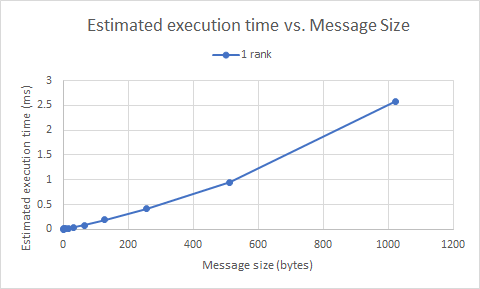
\includegraphics[width=0.45\linewidth]{exe_time_vs_messsage_size_rank_1.png}
}
\hspace*{\fill}
\subfloat[Rank 2]{
  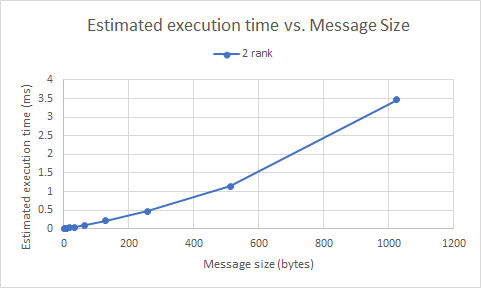
\includegraphics[width=0.45\linewidth]{exe_time_vs_messsage_size_rank_2.png}
}
\hspace{0mm}
\subfloat[Rank 3]{
  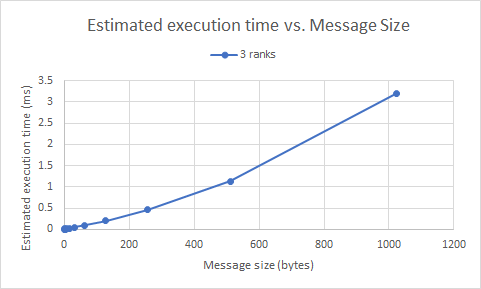
\includegraphics[width=0.4\linewidth]{exe_time_vs_messsage_size_rank_3.png}
}
\hspace*{\fill}
\subfloat[Rank 4]{
  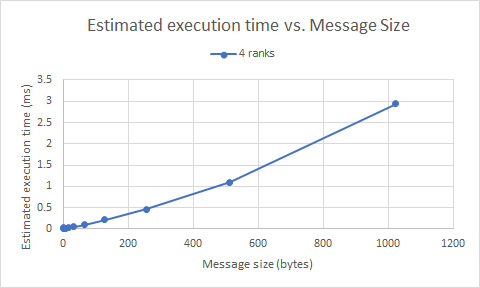
\includegraphics[width=0.45\linewidth]{exe_time_vs_messsage_size_rank_4.png}
}
\hspace{0mm}
\subfloat[Rank 5]{
  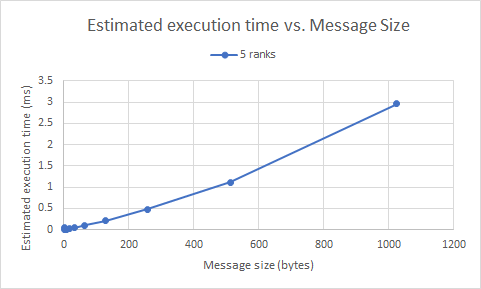
\includegraphics[width=0.45\linewidth]{exe_time_vs_messsage_size_rank_5.png}
}
\hspace*{\fill}
\subfloat[Rank 6]{
  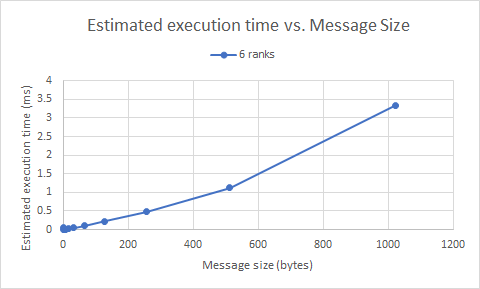
\includegraphics[width=0.45\linewidth]{exe_time_vs_messsage_size_rank_6.png}
}
\caption{Estimated execution time vs message size along different ranks.}
\end{figure*}

Figure 2 shows the result comparison of estimated execution time across different ranks versus message size and number of ranks. Note that the green column in Figure 2(b) represents the result from running on 2 nodes with each nodes having 6 MPI ranks.

\begin{figure*}[h!]
\hspace{0mm}
\subfloat[Comparison of estimated execution time vs message size across different ranks.]{
	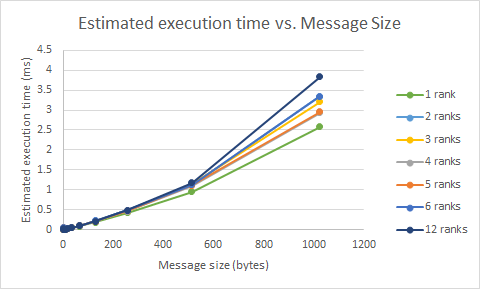
\includegraphics[width=0.5\linewidth]{estimated_execution_time_vs_message_size.png}
}
\hspace*{\fill}
\subfloat[Estimated execution time in relation to ranks]{
	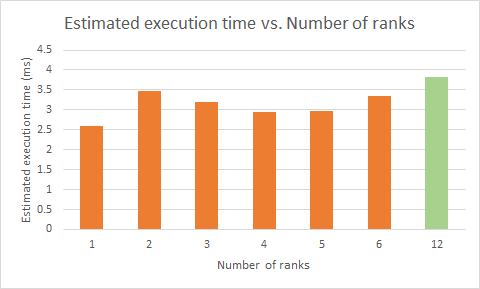
\includegraphics[width=0.5\linewidth]{estimated_execution_time_vs_number_of_ranks_1.png}
}
\caption{The relationship between message sizes and number of ranks to estimated execution time.}
\end{figure*}


\begin{figure}[h]
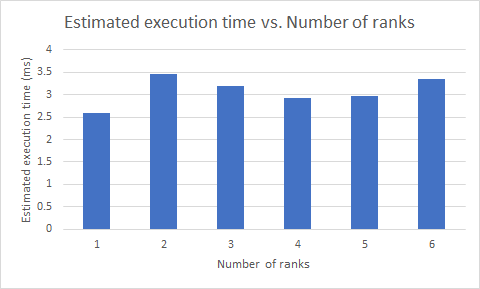
\includegraphics[width=0.5\textwidth]{estimated_execution_time_vs_number_of_ranks.png}
\caption{An alternative interpretation of the relations between estimated execution time and the number of ranks.}
\end{figure}
Strong scaling result is shown in the figure below.

\begin{figure}[H]
\centering
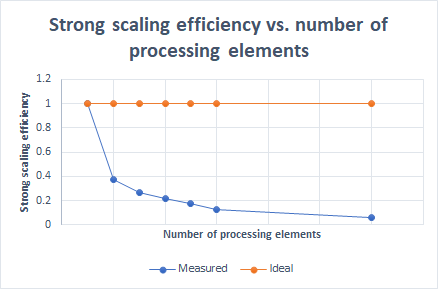
\includegraphics[width=\linewidth]{strong.png}
\caption{Strong scaling results}
\end{figure}

It can be observed that the strong scaling results are not very good but this is as expected. The overhead for the algorithm and communication increases as the number of processes increases and takes us to this result. It could be hard to reduce this part and we hadn't figure out how to do so.

And below is the weak scaling results.

\begin{figure}[H]
\centering
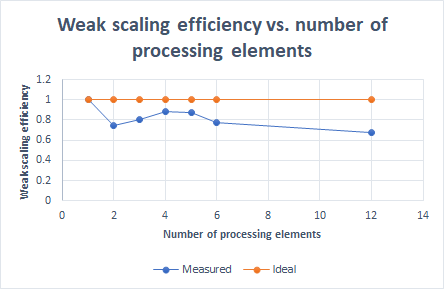
\includegraphics[width=\linewidth]{weak.png}
\caption{Weak scaling results}
\end{figure}

This result is better than the strong scaling result. In the sense that we didn't see significant drop in weak scaling efficiency as that in the strong scaling. Note that here is still a trend of dropping in the weak scaling efficiency.


\section{Conclusion and Future works} \label{conclusion}
% Conclusion and future works

In this work we perform benchmarking on four different parallel models to evaluate the perforamnce of the CUDA-aided Game of Life program. The GPU-accelerated program is integrated with MPI's communication mechanism to effectively manage the memory access as well as transfering among different nodes. 

For future works, there are two possible extensions on the program to study how different mechanism may further improve or deteriorate the performance of the current version of Game of Life program. The first possible direction is to incorporate multithreading to the current version to observe how sharing resources on the same node may affect the message communication, and another possible study involves the execution of the same GPU-accelerated program on different topologies such as the Fat Tree \cite{leiserson1985fat}, Dragonfly \cite{kim2009cost} or Slimfly \cite{wolfe2016modeling} networks to investigate the difference in performance described with the mentioned parallel models. 

\section{Acknowledgments}





%%
%% The next two lines define the bibliography style to be used, and
%% the bibliography file.
\bibliographystyle{ACM-Reference-Format}
\bibliography{references}



\end{document}
\endinput
%%
%% End of file `sample-authordraft.tex'.
